% ---------------------------------------------------------------------------
\section{Hepburn System}\jsec{ヘボン式}
%[o] LABEL
\label{sec:Hepburn}
\label{sec:HepburnSystem}
\label{sec:OlderHepburnSystem}
\label{sec:NewerHepburnSystem}
% [o] INDEX
\ifor{Hepburn system}{ヘボン式}{へぼんしき}{Hepburn System}
\ifor{Hepburn system!older}{標準ヘボン式ローマ字}{ひょうじゅん・へぼん・ろまあじ}{Hepburn System!altes}
\ifor{Hepburn system!newer}{修正ヘボン式ローマ字}{しゅうせい・へぼんしき・ろうまじ}{Hepburn System!neueres}
\ithree{James Curtis Hepburn}{James Curtis Hepburn}{James Curtis Hepburn}

\newcommand{\lhepburnsystem}{\ivoc{Hepburn system}{ヘボン式}{へぼんしき}{Hepburn System}}
\newcommand{\loldhepburnsystem}{\ivoc{old Hepburn system}{標準ヘボン式ローマ字}{ひょうじゅん・へぼん・ろまあじ}{altes Hepburn System}}
\newcommand{\lnewhepburnsystem}{\ivoc{new Hepburn system}{修正ヘボン式ローマ字}{しゅうせい・へぼんしき・ろうまじ}{neues Hepburn System}}

\begin{tabular}{lr}
\begin{minipage}{10.5cm}

The \lhepburnsystem{} is one of the two most important transcription systems
for the Japanese written \hyperref[sec:Mora]{morae} based language. The
\textbf{Hepburn system} is the most used system worldwide and in Japan.

The word {ヘボン} /hebon/ is an old writing of the name \textbf{Hepburn}, a US
American physician, translator, educator and a Christian missionary, who used
the transcription system in his first Japanese English Dictionary (3rd ed.) in
1867.

There are mainly two different variants: The \loldhepburnsystem{} variant,
which is used for signs at train stations. And the newer variant the
\lnewhepburnsystem{} which is used as a revised system since 1954 in Kenkyusha
dictionaries. Most western scientists are using this system. This system is
also used in this book.

\Link \href{https://en.wikipedia.org/wiki/James_Curtis_Hepburn}{Hepburn}

\end{minipage}
&
\raisebox{-.47\height}{
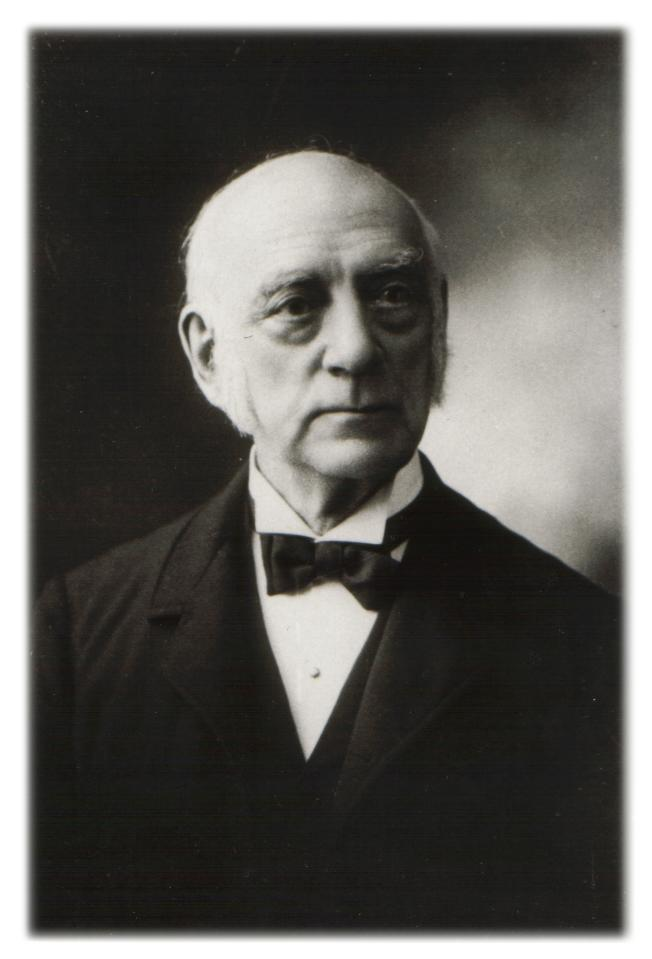
\includegraphics[scale=0.5,trim= 00 00 00 00]{../share/ei/James_Curtis_Hepburn.jpg}}
\\
\end{tabular}


